\documentclass[12pt]{article}
\usepackage[T1]{fontenc}
\usepackage[utf8]{inputenc}%\usepackage[latin1]{inputenc}
\DeclareUnicodeCharacter{0301}{\'{e}}
\usepackage[brazilian]{babel}
\usepackage{graphicx}
\usepackage{hyperref}
\usepackage{indentfirst}
\hypersetup{
  setpagesize  = false,
  colorlinks   = true,    % Colours links instead of ugly boxes
  urlcolor     = blue,    % Colour for external hyperlinks
  linkcolor    = blue,   % Colour of internal links
  citecolor    = blue    % Colour of citations
}
\urlstyle{same} 

\usepackage{authblk}
\usepackage{geometry}
\usepackage{setspace}
\singlespacing  %Setar espaçamento simples
\usepackage{verbatim}
\usepackage[utf8]{inputenc}
\usepackage{amsmath}
\usepackage{amssymb}
\usepackage{gensymb}
\usepackage{verbatim} % env for block comment 
\usepackage{ragged2e} % para usar flusleft
\usepackage[brazilian]{babel}
\usepackage{minted}
\usemintedstyle{tango}
\usepackage{amsfonts}
\usepackage{cancel}


\usepackage[sorting=none]{biblatex}
\addbibresource{referencias.bib}

\setcounter{page}{1} % página inicial do artigo
%==========================================================================
% Margens e tamanho da página
%==========================================================================
\setlength{\paperwidth}{19cm}\setlength{\paperheight}{29cm}
\setlength{\textwidth}{16cm}\setlength{\textheight}{25.4cm}
\setlength{\oddsidemargin}{1.5cm}
\setlength{\headheight}{\baselineskip}
\setlength{\topmargin}{.5cm}
%\setlength{\headsep}{2cm}\addtolength{\headsep}{-\headheight}
\setlength{\footskip}{2cm}\addtolength{\footskip}{.5\baselineskip}
\addtolength{\topmargin}{-1in}
\addtolength{\oddsidemargin}{-1in}
\setlength{\evensidemargin}{\oddsidemargin}
%==========================================================================
% Definições diversas
%==========================================================================
\setlength{\parindent}{1cm}
\newcommand{\abstractinenglishname}{Abstract}
\newcommand{\keywordsportugues}{Palavras-chave}
\newcommand{\keywordsenglishname}{Keywords}




%==========================================================================
% Artigo
%==========================================================================

\title {Detecção e Medição Automatizada de Trincas em Estruturas de Aço Usando Aprendizado Profundo e Visão Computacional}

%==========================================================================
% Não editar o cabeçalho
%==========================================================================
\usepackage{fancyhdr}
\fancyhf{}
\fancyhead[L]{\small Rangel Ávila Barroso - Pré-Projeto de Mestrado UFMG}
%==========================================================================
% Não editar o cabeçalho
%==========================================================================
\fancyhead[R]{\thepage}
\pagestyle{fancy}

\begin{document}

\begin{center}
\Large\bfseries
Visão Computacional e Aprendizado Profundo Semissupervisionado para Detecção e Medição de Trincas em Estruturas de Aço
\end{center}

\section{Introdução}

A nucleação e a propagação de trincas em estruturas de aço submetidas a carregamentos cíclicos representam o modo de falha predominante em máquinas, componentes mecânicos e construções metálicas, constituindo cerca de 90\% das falhas em serviço \cite{1hosford2010solid}. Nesses casos, estima-se que 20-40\% da vida útil dos componentes seja consumida na fase denominada crescimento estável da trinca \cite{2newman1998merging}, estágio em que o aumento do dano possui maior previsibilidade e dimensões detectáveis, tornando imperativo o uso de técnicas para identificar e monitorar esse tipo de defeito. 

Para isso, os processos de SHM (\textit{Structural Health Monitoring}) desempenham um papel fundamental, pois contemplam atividades de acompanhamento constante da integridade estrutural. No entanto, o SHM ainda é realizado, em grande parte, de forma manual, através de inspeções visuais ou a partir de ensaios não destrutivos. Esses métodos oferecem baixa escalabilidade, além de estarem suscetíveis a erros humanos e à dificuldade no acesso de alguns locais, comprometendo a precisão e a eficácia desses procedimentos.

O uso de técnicas de visão computacional como uma alternativa para o SHM na detecção de trincas vem se destacando nos últimos anos, principalmente no acompanhamento de estruturas de concreto como pontes, viadutos, represas e pavimentos rodoviários \cite{14konig2022s}. Porém, o monitoramento de estruturas de aço apresenta obstáculos específicos, como apontado por \textcite{12li2021deep}:
\begin{itemize}
    \item \textbf{Variabilidade ambiental:} Condições precárias de iluminação, reflexos e texturas metálicas diversas (presença de corrosão ou camadas de tinta);
    \item \textbf{Variabilidade geométrica:} Geometrias complexas, presença de soldas e/ou ligações parafusadas;
    \item \textbf{Escassez de dados:} \textit{Datasets} públicos e rotulados para trincas em aço são limitados em comparação a estruturas de concreto.
\end{itemize}

Além da identificação das trincas, é de suma importância a medição de suas propriedades geométricas, como comprimento, largura e orientação, uma vez que essas informações constituem os \textit{inputs} de modelos empíricos para predição de vida remanescente \cite{5kala2006sensitivity}. Esses modelos são extremamente sensíveis aos parâmetros geométricos da trinca, o que pode aumentar as incertezas no cálculo e comprometer a confiabilidade da predição. Uma alternativa para mitigar esses erros consiste na implementação de um sistema de monitoramento automatizado, utilizando redes neurais convolucionais profundas (\textit{Deep Convolutional Neural Networks}, D-CNNs) de segmentação semântica, complementadas por etapas de pós-processamento baseadas em operações morfológicas para obtenção das características geométricas das trincas a partir dos mapas semânticos \cite{14konig2022s}.

Este projeto tem como objetivo desenvolver um modelo de visão computacional e aprendizado profundo para detecção e quantificação de trincas em estruturas metálicas. A proposta envolve a combinação de dados públicos e rotulados provenientes de outros tipos de superfícies e dados não rotulados de estruturas de aço, utilizando técnicas de aprendizado semissupervisionado. Espera-se que o modelo seja versátil e eficiente, permitindo sua implementação em câmeras industriais, UAVs (\textit{Unmanned Aerial Vehicles}) ou dispositivos portáteis. 

\section{Referencial Teórico}

A partir de 2012, a utilização de D-CNNs, combinadas com GPUs modernas e grandes volumes de dados, revolucionou a classificação de imagens em larga escala, como demonstrado pela AlexNet \cite{8krizhevsky2017imagenet}. Em 2014, a arquitetura R-CNN (\textit{Regions with Convolutional Neural Networks}) representou um novo avanço ao aplicar redes convolucionais para cada região de interesse dentro de uma imagem. No entanto, esta abordagem apresentava limitações para detecção de objetos em tempo real devido ao seu alto custo computacional \cite{9girshick2014rich}.

Para superar essas limitações, a arquitetura YOLO (\textit{You Only Look Once}) foi desenvolvida por Joseph Redmon et al. \cite{10redmon2016you} em 2015, demonstrando um aumento significativo de desempenho na detecção de objetos ao prever simultaneamente \textit{bounding boxes} e classificações em uma única avaliação completa da imagem. No mesmo ano, a arquitetura U-Net foi introduzida para segmentação de imagens biomédicas \cite{11ronneberger2015u}, estabelecendo um modelo capaz de classificar e extrair informações quantitativas de objetos a partir de um conjunto de dados reduzido, dada a escassez de imagens para treinamento no contexto biomédico. Esse processo de quantificação, chamado de segmentação semântica, atribui a cada pixel de uma imagem um rótulo correspondente à classe do objeto ou região a que pertence (cor, textura, vizinhança etc.). Dessa forma, mapas de segmentação semântica são gerados, onde cada pixel da imagem reflete sua classe semântica. 

No contexto da medição de trincas, a segmentação binária (trinca/não trinca) vem sendo utilizada para gerar mapas detalhados pixel-a-pixel dos defeitos \cite{13bhowmick2020vision}. A partir desses mapas, é possível quantificar características como comprimento, largura média, área e orientação da trinca através de operações morfológicas, viabilizando o monitoramento automatizado da estrutura de interesse. Além da obtenção dessas informações, outros tipos de operações podem ser implementados, como filtros para a redução de ruídos no mapa, ou o preenchimento de lacunas artificiais e refinamento de bordas.

Entretanto, observa-se uma lacuna na literatura quanto  à aplicação de \textit{pipelines} adaptados às estruturas metálicas, principalmente em ambientes industriais. Variações reais como corrosão, pintura, existência de soldas ou ligações parafusadas e ruídos da aquisição dos dados afetam significativamente a eficácia dos modelos \cite{12li2021deep}. Além disso,  \textcite{14konig2022s} e \textcite{15wang2021semi} destacam que o estado da arte da segmentação semântica de trincas baseia-se fortemente em aprendizado supervisionado, exigindo grande quantidade de dados rotulados manualmente pixel-a-pixel para treinamento dos modelos, o que torna a etapa de pré-processamento trabalhosa e custosa. 

Outro desafio encontrado na elaboração de modelos treinados a partir de um conjunto de dados reduzido é o \textit{overfitting}, fenômeno em que o modelo apresenta um excesso de parâmetros para o \textit{dataset} de treinamento, prejudicando sua generalização \cite{6shorten2019survey}. Para mitigar esse efeito, técnicas de \textit{data augmentation} são essenciais para aumentar a diversidade do conjunto de dados e diminuir possíveis vieses. Esse processo consiste em realizar transformações nas imagens como: rotação, espelhamento, escalonamento (alterações de \textit{zoom}), cortes aleatórios, além de alterações nas cores, na iluminação e no desfoque.

Tendo em vista o potencial da visão computacional nos processos de SHM e as atuais limitações observadas na sua adaptação para estruturas metálicas, este projeto irá propor uma arquitetura adaptada para detecção e medição de trincas por meio de aprendizado semissupervisionado, mesclando conjuntos de dados rotulados públicos para estruturas de concreto / pavimentos rodoviários com um \textit{dataset} não rotulado de estruturas de aço. O modelo integrará técnicas de classificação e segmentação semântica com etapas de pós-processamento através de operações morfológicas %(REF17)% 
para aumentar a qualidade dos mapas semânticos e extrair informações geométricas relevantes para determinar a severidade das trincas, incluindo: seu comprimento, largura média e orientação.

\section{Metodologia}

O fluxograma do projeto é apresentado na \autoref{fig1}. São propostas quatro etapas principais, que serão executadas em paralelo aos estudos aprofundados para a elaboração do trabalho e à realização das disciplinas indicadas na \autoref{Cronograma}. O detalhamento das atividades previstas para cada uma dessas etapas é apresentado a seguir.

%\setlength{\textfloatsep}{5pt} % Space between float and text
%\setlength{\floatsep}{5pt}    % Space between floats
%\setlength{\intextsep}{5pt}   % Space for in-text floats
\begin{figure}[h]
  \centering
  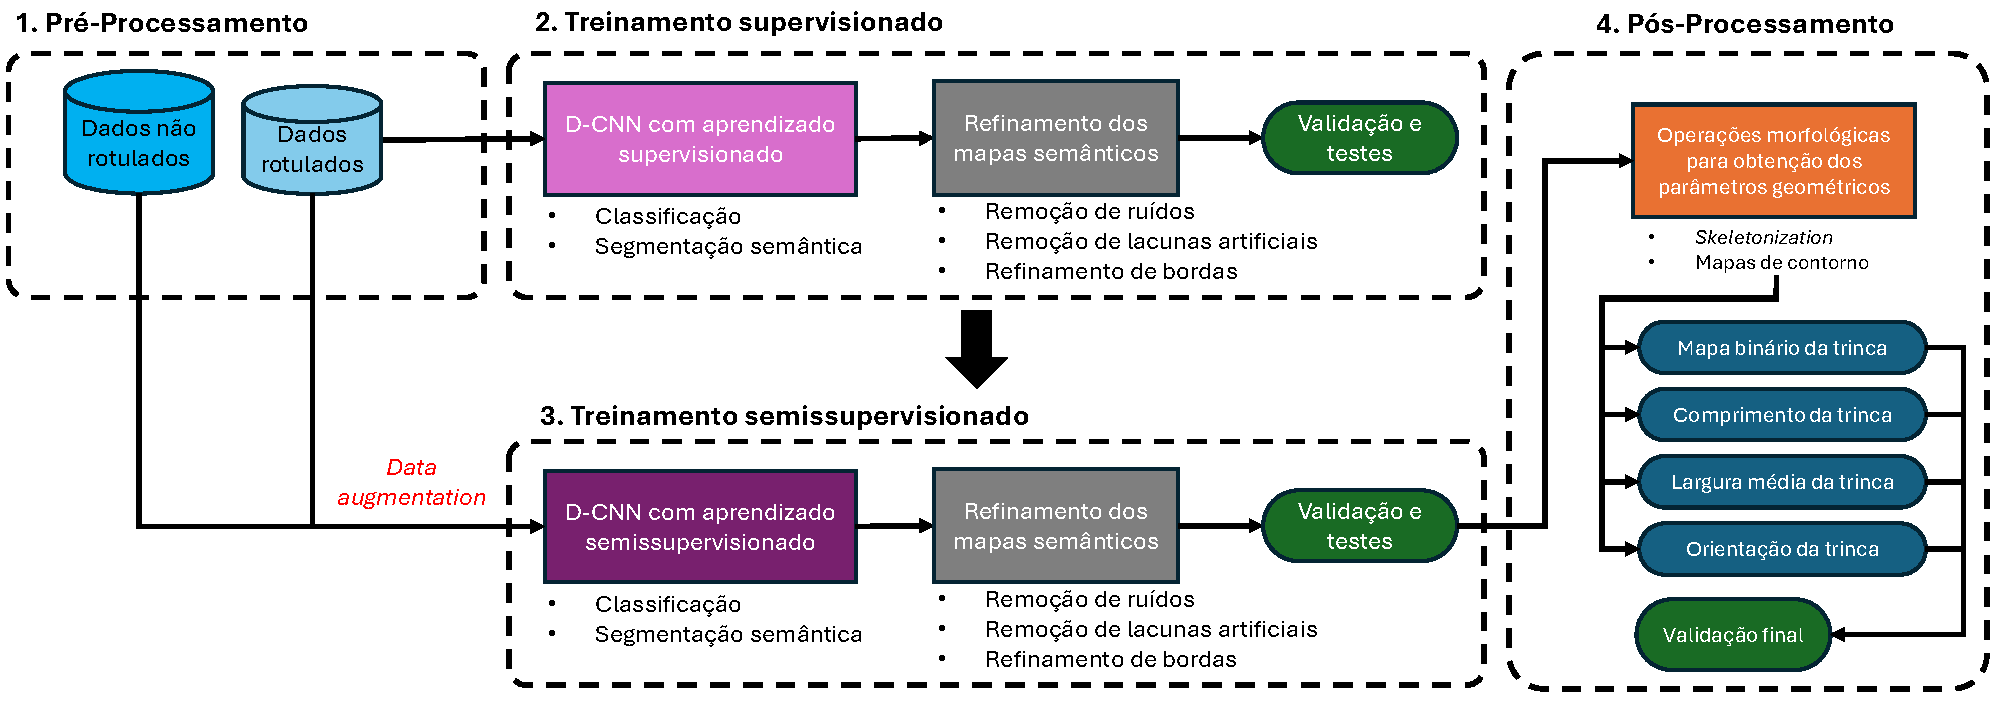
\includegraphics[width=\textwidth]{imagens/metodologia_PPP2_cropped.pdf}
  \setlength{\abovecaptionskip}{0pt} % valor padrão é ~10pt
  \vspace{-10pt}
  \caption{Fluxograma metodológico do projeto.}
  \label{fig1}
\end{figure}
%\begin{figure}[H]
%\begin{center}
%\includegraphics[width=16 cm]{imagens/fluxograma_metodologia.png}
%\caption{Fluxograma metodológico do projeto}
%\label{fig1}
%\vspace{-20pt}
%\end{center}
%\end{figure}]
\vspace{-5pt}
\subsection{Pré-Processamento}
A preparação dos dados consistirá em três atividades: 1) aquisição dos dados públicos rotulados, 2) aquisição dos dados não rotulados de estruturas de aço e 3) realização de \textit{data augmentation}. Para a primeira etapa, \textcite{14konig2022s} indica diversos conjuntos de dados rotulados para estruturas de concreto e pavimentos rodoviários disponíveis online. Para a obtenção de imagens não rotuladas de trincas em estruturas de aço, será conduzida uma busca aprofundada na internet, além do envio de solicitações para empresas de consultoria em engenharia e inspeção de ativos industriais. 

Para o conjunto de dados rotulado, serão definidas as partições destinadas aos testes e treinamento. %(REF18) 
Do conjunto de treinamento, uma fração será alocada para a validação do modelo supervisionado (e seus respectivos mapas semânticos \textit{ground truth}) e o restante para o treinamento em si do modelo. Ainda, serão efetuadas transformações nas imagens via \textit{data augmentation}, como rotações, \textit{flipping}, injeção de ruído e outras técnicas apresentadas por \textcite{6shorten2019survey}.

\subsection{Treinamento Supervisionado}

Nesta etapa, o \textit{dataset} rotulado será utilizado para o treinamento supervisionado da D-CNN. Será realizada uma pesquisa aprofundada para a definição da arquitetura mais adequada à finalidade do projeto. Os mapas semânticos serão refinados através de técnicas de processamento de imagem, que incluem: remoção de ruídos, remoção de lacunas artificiais e refinamento de bordas, aumentando a qualidade dos resultados. Para a validação deste modelo, serão avaliadas abordagens como \textit{F1 Score} \cite{15wang2021semi}, IoU (\textit{Intersect over Union}) e \textit{Dice Score} \cite{18shamsabadi2024efficient}, além de outras métricas consolidadas na literatura.

\subsection{Treinamento Semissupervisionado}

O treinamento semissupervisionado será definido a partir de uma pesquisa aprofundada sobre o estado da arte na segmentação de trincas. Serão avaliadas possibilidades como: \textit{consistency regularisation}, \textit{self-training} com \textit{pseudo-labelling}, interfaces \textit{teacher-student}, além da integração dessas abordagens \cite{18shamsabadi2024efficient}. As atividades de refinamento dos mapas semânticos e validação do modelo serão similares às da etapa de treinamento supervisionado.

\subsection{Pós-Processamento}

Para extrair os parâmetros geométricos de interesse do mapa semântico das trincas, serão realizadas operações morfológicas de \textit{skeletonization} (diminuição sucessiva de bordas até alcançar uma trinca com um pixel de largura) \cite{13bhowmick2020vision} e elaboração dos mapas de contorno (extrair apenas os contornos da trinca). A partir desses resultados, algoritmos para cálculo do comprimento e orientação da trinca serão implementados. Também será realizada uma pesquisa sobre métodos para aquisição dos fatores de escala, necessários para a obtenção das dimensões físicas reais das trincas (pixel para milímetros, por exemplo). A validação final do modelo será realizada a partir de um \textit{set} pequeno de trincas com suas características físicas anotadas manualmente.


\section{Cronograma}\label{Cronograma}

O cronograma evidenciado na \autoref{fig2} destaca as tarefas a serem realizadas durante o Mestrado, divididas entre realização de disciplinas, estudo aprofundado do projeto e a elaboração do projeto em si. A ordem das disciplinas foi planejada de forma a complementar o estudo aprofundado acerca do projeto e a promover um sequenciamento do aprendizado nas áreas de Aprendizado de Máquina, Visão Computacional, Processamento de Imagens e Inteligência Artificial.

%\begin{enumerate}
    %\item Projeto e Análise de Algoritmos
    %\item Aprendizado de Máquina
   % \item Aprendizado Profundo
   % \item Visão Computacional
   % \item Processamento Digital de Imagens
   % \item Tópicos em Inteligência Artificial
   % \item Estágio em Docência
%\end{enumerate}

%\setlength{\textfloatsep}{5pt} % Space between float and text
%\setlength{\floatsep}{5pt}    % Space between floats
%\setlength{\intextsep}{5pt}   % Space for in-text floats
\begin{figure}[H]
  \centering
  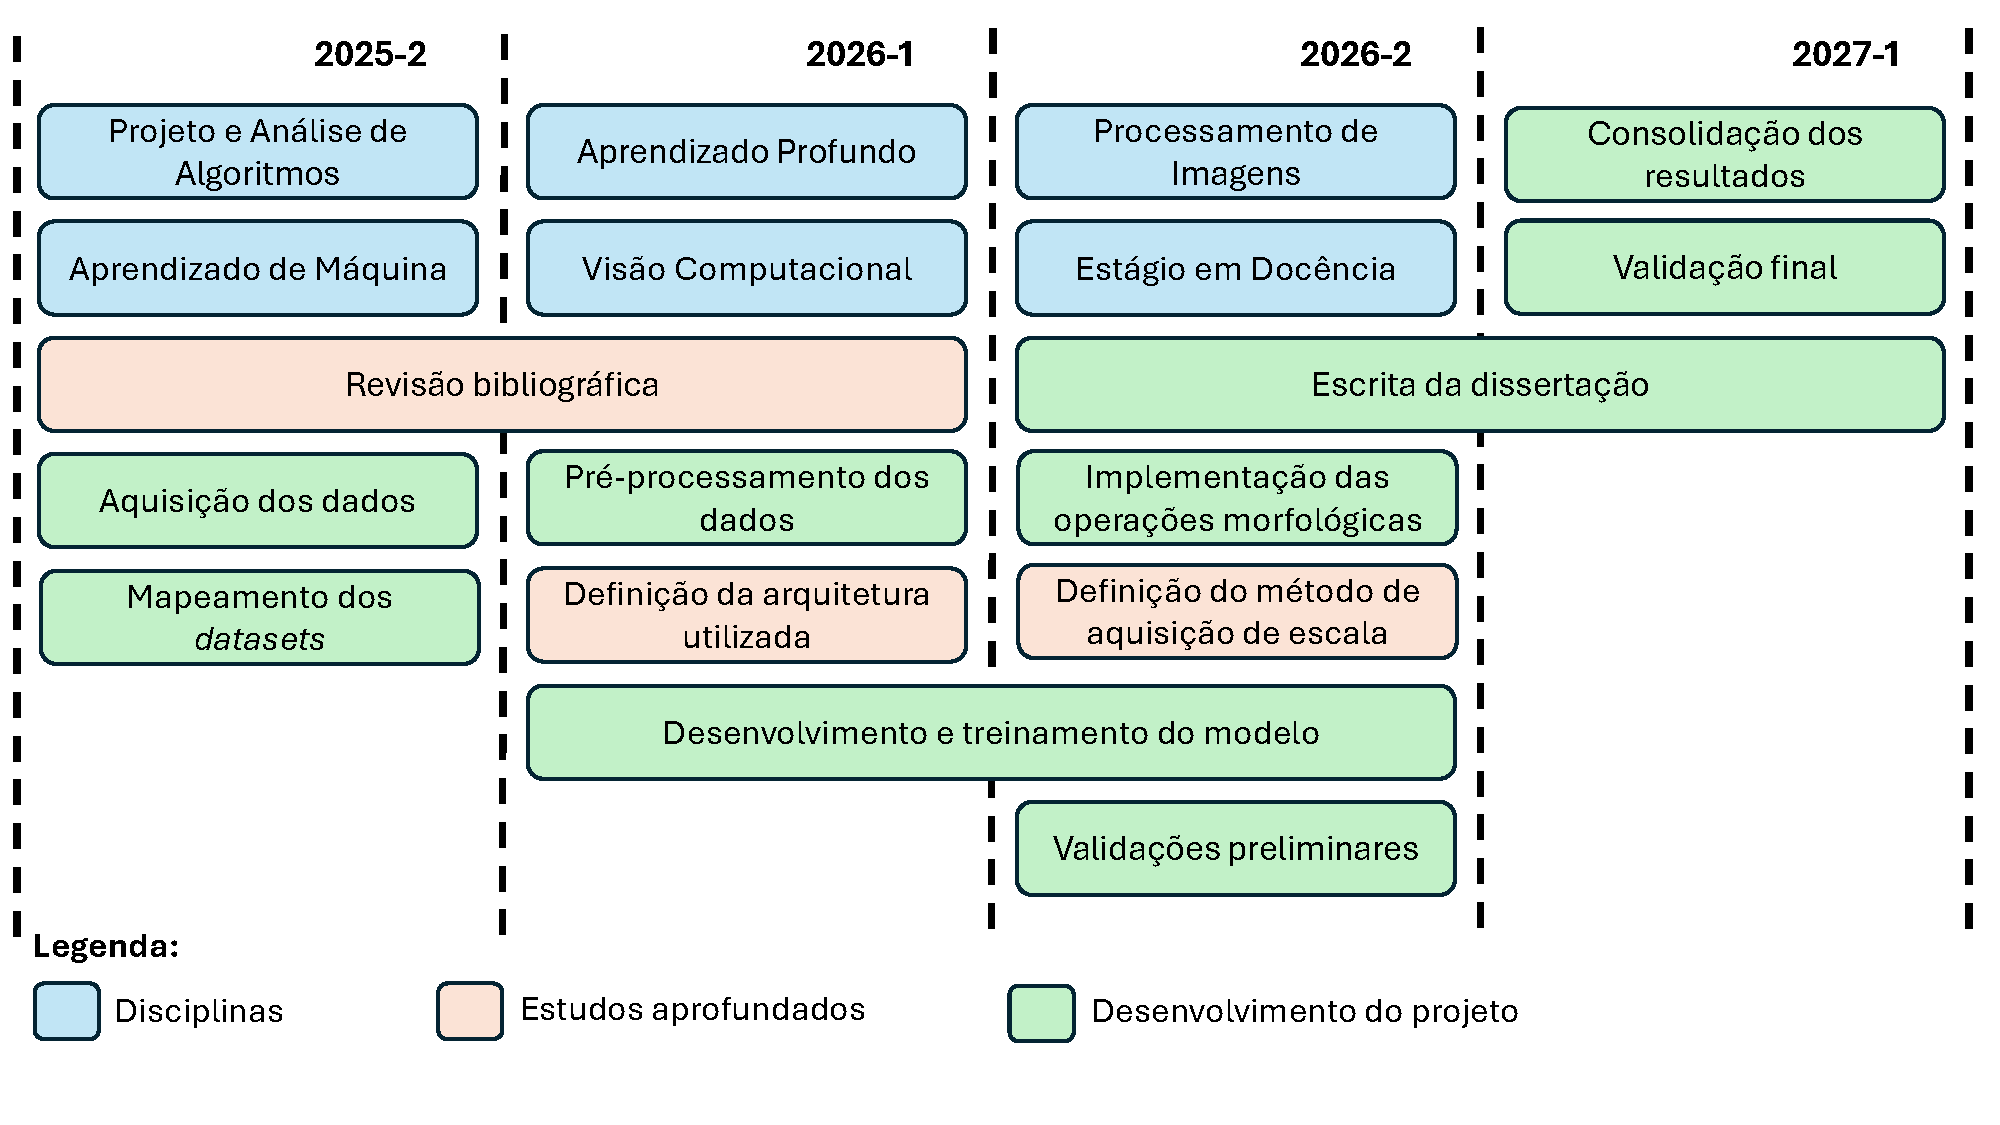
\includegraphics[width=0.75\textwidth]{imagens/Cronograma_PPP.pdf}
  \setlength{\abovecaptionskip}{0pt} % valor padrão é ~10pt
  \vspace{-10pt}
  \caption{Cronograma do Mestrado.}
  \label{fig2}
\end{figure}

%\textit{Observação: O GPT-4o com o recurso de memória foi utilizado antes do início do projeto, para auxiliar na decisão do tema baseado nas preferências, áreas de atuação e interesses do autor. A Perplexity AI foi utilizada como ferramenta de busca inteligente no início do  pesquisa bibliográfica, filtrando diversos artigos sobre o tema escolhido de forma assertiva. A única ferramenta de correção ortográfica utilizada foi a nativa do Overleaf (versão gratuita).}
\printbibliography

\end{document} 